\documentclass[border=6pt]{standalone}
\usepackage{tikz}
\usetikzlibrary{arrows.meta,positioning,calc}
\begin{document}
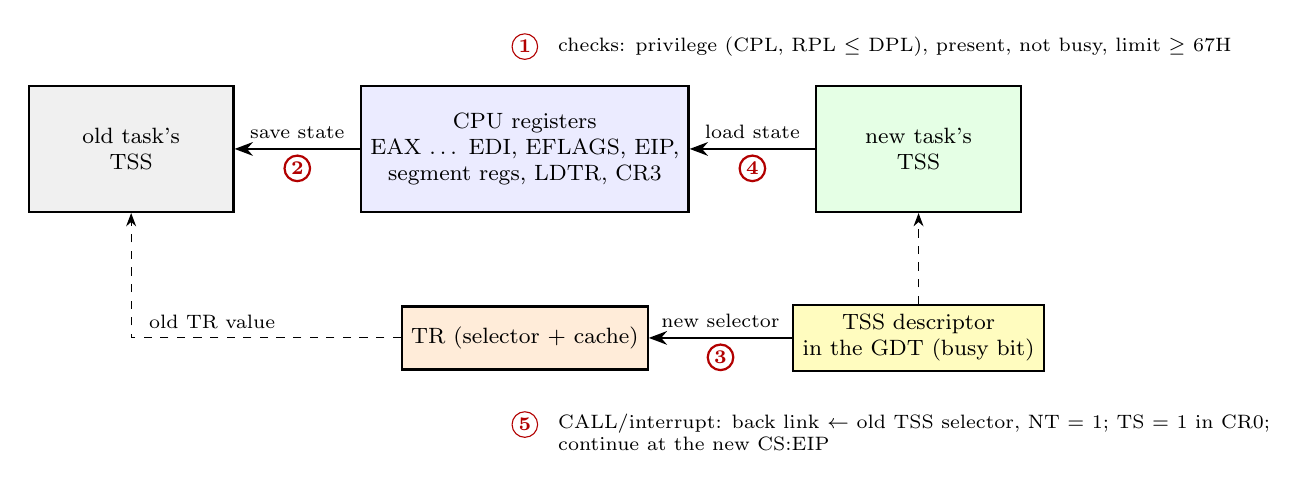
\begin{tikzpicture}[>=Stealth,font=\small,
 b/.style={draw,thick,align=center,font=\footnotesize,minimum height=0.8cm},
 s/.style={circle,draw=red!70!black,fill=white,font=\scriptsize\bfseries,text=red!70!black,inner sep=1pt}]
\node[b,fill=blue!8,minimum width=3.0cm,minimum height=1.6cm] (cpu) at (5,0) {CPU registers\\EAX \dots\ EDI, EFLAGS, EIP,\\segment regs, LDTR, CR3};
\node[b,fill=gray!12,minimum width=2.6cm,minimum height=1.6cm] (old) at (0,0) {old task's\\TSS};
\node[b,fill=green!10,minimum width=2.6cm,minimum height=1.6cm] (new) at (10,0) {new task's\\TSS};
\node[b,fill=orange!15,minimum width=2.4cm] (tr) at (5,-2.4) {TR (selector + cache)};
\node[b,fill=yellow!25,minimum width=2.6cm] (gdt) at (10,-2.4) {TSS descriptor\\in the GDT (busy bit)};
\draw[->,thick] (cpu.west) -- (old.east) node[midway,above,font=\scriptsize]{save state} node[midway,below=2pt,s]{2};
\draw[->,thick] (new.west) -- (cpu.east) node[midway,above,font=\scriptsize]{load state} node[midway,below=2pt,s]{4};
\draw[->,thick] (gdt.west) -- (tr.east) node[midway,above,font=\scriptsize]{new selector} node[midway,below=2pt,s]{3};
\draw[->,dashed] (tr.west) -| (old.south) node[pos=0.35,above,font=\scriptsize]{old TR value};
\draw[->,dashed] (gdt.north) -- (new.south);
\node[s] at (5,1.3) {1};
\node[font=\scriptsize,anchor=west] at (5.3,1.3) {checks: privilege (CPL, RPL $\le$ DPL), present, not busy, limit $\ge$ 67H};
\node[s] at (5,-3.5) {5};
\node[font=\scriptsize,anchor=west,align=left] at (5.3,-3.6) {CALL/interrupt: back link $\leftarrow$ old TSS selector, NT = 1; TS = 1 in CR0;\\continue at the new CS:EIP};
\end{tikzpicture}
\end{document}
